\chapter{Proteins: Folded Molecular Machines}

\begin{kaichang}
Crack a raw egg into a clear glass. Its white is a translucent, thin, flowing liquid. Now boil and peel another egg: the white has become one firm, elastic, white mass holding the yolk securely at its center.

Here is a question worth pausing over. Frozen water melts again when heated; melted chocolate solidifies again when cooled. But put cooked egg white in a refrigerator, soak it in water, or recite any spell, and it never becomes that transparent liquid again. What did heating do to make the change run in only one direction?

Write down your guess. By this chapter's end, you will not only answer this question, but understand how your hair, muscles, flowing blood, wound scabs, and the soy milk used for tofu are all tricks performed by one family of molecules---proteins.
\end{kaichang}

\section{What Egg White, Hair, and Tofu Share}

First, consider everyday ``protein moments'':

\begin{itemize}[itemsep=2pt]
\item Boiling an egg turns its white from a transparent liquid into a white solid;
\item A hair salon applies chemicals and heat to set a perm, keeping straight hair curly for months;
\item A spoonful of brine (mainly containing magnesium chloride) coagulates a pot of soy milk into tofu;
\item Milk left too long becomes sour and forms fluffy little clumps;
\item Broth from stewed meat sets into jelly when cooled and melts into delicious liquid in your mouth;
\item A cut finger's blood soon clots, blocking bacteria.
\end{itemize}

Apparently unrelated, these phenomena share a molecular family. Egg white contains mainly ovalbumin; hair and nails mainly keratin; soy milk contains soy proteins; meat jelly is heat-unraveled collagen; and clotting depends on fibrinogen. Remove water from your body mass, and roughly half of what remains is protein: muscle, skin, hair, the framework in bones, and blood's oxygen-carrying hemoglobin all enter this account.

The last two chapters introduced carbohydrates (Chapter 46) and lipids (Chapter 47): carbohydrates resemble standardized fuel blocks and building materials, while lipids are water-shy energy stores and wall materials. Proteins have a different role: they are \textbf{working machines}. Carbohydrates can burn for energy and lipids can be stored, but almost every protein has a specific job---transport, support, recognition, defense, catalysis, or contraction. A city needs more than fuel and bricks; it also needs cranes, conveyors, guards, and wrenches. Proteins are the cellular city's complete machinery.

Machines need shapes. A crane cannot be a puddle of molten iron, nor a wrench a tangle of cotton thread. This chapter follows where a protein machine's shape comes from and why it can be lost.

\section{Twenty Parts in One Long Chain}

Zoom to the molecular level. However complex a protein is, dismantling it completely yields repetitions of one kind of part: \textbf{amino acids}.

The name already reveals their structure (Chapter 37 discussed functional-group naming): an amino group (\chem{{-}NH_2}, nitrogen-containing and somewhat basic) at one end, and a carboxyl group (\chem{{-}COOH}, proton-donating and somewhat acidic) at the other. Between them sits a carbon also attached to a hydrogen and a \textbf{side chain}. All amino acids have the same framework; only side chains differ, like twenty LEGO pieces with identical sockets but different shapes.

The human body uses 20 standard parts to build proteins. By side-chain temperament, they fall roughly into several groups:

\begin{itemize}[itemsep=2pt]
\item \textbf{Water-shy}: hydrocarbon chains or rings that behave like oil and avoid water. Leucine and phenylalanine belong here.
\item \textbf{Water-loving}: polar groups such as hydroxyls and amino groups that hydrogen-bond with water and favor aqueous surroundings. Serine and glutamine belong here.
\item \textbf{Charged}: side chains carrying outright positive or negative charge at bodily-fluid pH. Lysine is positive; glutamate is negative.
\item \textbf{Specialists}: cysteine has a terminal sulfhydryl (\chem{{-}SH}). When two cysteines meet, their sulfurs can join hands in a strong covalent bridge---a \textbf{disulfide bond}. Remember it: your curls depend on it.
\end{itemize}

How are the parts strung into chains? Through Chapter 38's condensation reaction: one amino acid's carboxyl meets the next one's amino group, expels water, and forms a carbon--nitrogen covalent bond. This has a special name: the \textbf{peptide bond}. Two amino acids condense into a dipeptide, three into a tripeptide, and dozens or hundreds into a \textbf{polypeptide chain}---the protein itself. A typical protein joins dozens to thousands of amino acids end to end, like a train with hundreds of cars sharing the same chassis but carrying different cargo.

The chain can also be dismantled: adding water hydrolyzes peptide bonds (Chapter 38), breaking the long chain into free amino acids. Your stomach and small intestine do this daily; we will revisit the full account in the misconceptions section.

Two earlier connections are worth noting. First, except in glycine, the central amino-acid carbon is chiral (Chapter 42), and life uses almost exclusively the left-handed half of the mirror pairs. A protein is assembled entirely from left-handed parts, making it highly selective about other molecules' handedness. Second, a protein is a polymer (Chapter 43), chained by condensation like nylon. But nylon repeats only one or two monomers, while proteins arrange 20 monomer types in unique sequences. Sequence is information.

\section{How a Chain Folds Itself into a Machine}

How does a floppy chain become a machine with a definite shape? It is not molded by someone; it \textbf{folds itself}. No blueprint worker is needed, only the chain, water, and Chapter 27's old rule: a system tends toward arrangements of lower free energy. Choose words carefully: the chain has no intention to fold. Through countless random twists, it samples energetically more favorable poses, which occur more often and persist longer.

Four influences drive folding:

\begin{itemize}[itemsep=2pt]
\item \textbf{The hydrophobic effect} (the main contributor). Water-shy side chains avoid exposure to water. As Chapter 47 explained, water molecules prefer less trouble: they let hydrophobic groups gather inside so they can freely hydrogen-bond. The chain closes like a sensitive plant, hiding water-shy side chains in its core and leaving water-loving ones outside---folding's overall steering wheel.
\item \textbf{Hydrogen bonds}. Backbone carbonyl oxygens and imino hydrogens hydrogen-bond, fixing sections into regular geometries: springlike \textbf{$\alpha$ helices} or straight, side-by-side, tilelike \textbf{$\beta$ sheets}. These recurring local structures are \textbf{secondary structure}.
\item \textbf{Ionic interactions (salt bridges)}. Positive and negative side chains attract across a gap like small magnets, fastening distant parts of the chain together.
\item \textbf{Disulfide bonds}. Two cysteine sulfurs form a genuine covalent bond, a structural ``rivet'' particularly resistant to heat and pulling. Keratin has many, making hair durable and hooves and horns hard.
\end{itemize}

The complete folded shape of one chain is \textbf{tertiary structure}---the individual machine. Some machines work only after joining together: folded chains, or subunits, assemble in fixed arrangements called \textbf{quaternary structure}. Hemoglobin combines four chains.

Thus proteins have four levels: primary amino-acid sequence, secondary local helices and sheets, tertiary whole-chain folding, and quaternary multisubunit assembly. Remember these levels, but especially their driving statement: \textbf{sequence determines folding, folding determines shape, and shape determines function}.

\begin{qiaoliang}
How extraordinary is folding? Calculate. Take a chain of 100 amino acids, short for a protein, and conservatively assume only three poses per amino acid. The whole chain has
\[3^{100} \approx 5\times 10^{47}\ \text{arrangements.}\]
Changing pose every $10^{-13}$ seconds---already absurdly fast---would require
\[5\times 10^{47}\times 10^{-13}\ \mathrm{s}=5\times 10^{34}\ \mathrm{s}\approx 1.6\times 10^{27}\ \text{years,}\]
to try them all, while the universe is only $1.4\times 10^{10}$ years old. Real proteins fold in milliseconds to seconds. The unavoidable conclusion: folding \textbf{is not an exhaustive random search}. Each correct twist lowers energy; correct contacts stabilize and guide the next step. Water flowing downhill does not randomly explore the entire map before finding the valley: it follows the slope. This ``energy slope'' is the key picture. A primary sequence is more than a parts list; it encodes the downhill route.
\end{qiaoliang}

\section{Drawing the Folding Plan}

Symbols arrive last. The general amino-acid formula writes the shared framework and represents the variable side chain as $\chem{R}$:

\[\chem{H_2N{-}CH(R){-}COOH}\]

Peptide-bond formation is written as condensation:

\[\chem{H_2N{-}CH(R_1){-}COOH} + \chem{H_2N{-}CH(R_2){-}COOH} \rightarrow \chem{H_2N{-}CH(R_1){-}CO{-}NH{-}CH(R_2){-}COOH} + \chem{H_2O}\]

The new central \chem{{-}CO{-}NH{-}} is the peptide linkage, actually Chapter 37's amide linkage under its protein-context name. It tends to be planar and resists rotation, like little rigid steel plates along a chain; flexibility comes from their connecting joints. This ``semirigid chain'' constrains much of folding's geometry.

A simple diagram connects the four levels:

\begin{center}
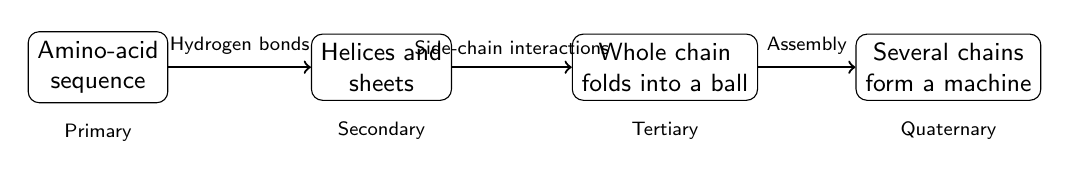
\begin{tikzpicture}[font=\small\sffamily]
\node[draw,rounded corners,align=center] (a) at (0,0) {Amino-acid\\sequence};
\node[draw,rounded corners,align=center] (b) at (3.6,0) {Helices and\\sheets};
\node[draw,rounded corners,align=center] (c) at (7.2,0) {Whole chain\\folds into a ball};
\node[draw,rounded corners,align=center] (d) at (10.8,0) {Several chains\\form a machine};
\draw[->,thick] (a) -- node[above=1pt]{\scriptsize Hydrogen bonds} (b);
\draw[->,thick] (b) -- node[above=1pt]{\scriptsize Side-chain interactions} (c);
\draw[->,thick] (c) -- node[above=1pt]{\scriptsize Assembly} (d);
\node[anchor=north] at ([yshift=-4pt]a.south) {\scriptsize Primary};
\node[anchor=north] at ([yshift=-4pt]b.south) {\scriptsize Secondary};
\node[anchor=north] at ([yshift=-4pt]c.south) {\scriptsize Tertiary};
\node[anchor=north] at ([yshift=-4pt]d.south) {\scriptsize Quaternary};
\end{tikzpicture}
\end{center}

This is a human-made representation: boxes and arrows aid thought. Real folding has no such tidy stage; it is a stew of molecular thermal motion with all processes occurring together.

\section{Shape Is Ability}

``Structure determines function'' is especially vivid in proteins. Look at five machines:

\textbf{Hemoglobin} is a courier. Each of its four chains (quaternary structure) holds a heme, whose central iron---the iron mentioned at Chapter 10's opening---gently grips an oxygen molecule. It collects oxygen where abundant in the lungs and releases it where scarce in tissues. Better still, one chain's oxygen binding slightly changes its shape, nudging its three neighbors to bind more readily. This cooperativity is a teamwork skill available through quaternary structure.

\textbf{Collagen} is a steel cable. Three chains twist into a rope-like triple helix. Its key trick: every third amino acid must be glycine, the smallest, with no bulky side chain, because only it fits the rope's center. These cables give skin, tendons, and bones toughness. The jelly in slow-cooked broth comes from prolonged heating unraveling the triple helices.

\textbf{Antibodies} are guards' radios. These Y-shaped molecules have antigen-recognizing sites at both arm tips, with billions of antibody types each recognizing particular targets; the tail calls immune cells to deal with them. Your body can custom-build antibodies for almost any unfamiliar intruder, a story for Volume III's immunity chapters. For now, remember that recognition precision comes from the close complementarity of folded shapes.

\textbf{Actin} is dismantlable scaffolding. Individual actin molecules are globular but join like beads into long fibers and disassemble when needed. Muscle contraction, crawling cells, and cells splitting in two all rely on these ``self-assembling ropes'' and their motor-protein partners.

\textbf{Ion channels} are pipes with access controls. Embedded across a membrane, they fold into a through-pore whose charge and width admit particular ions, such as sodium or potassium, with gates that open and close. Nerve signals depend on their switching rhythm. Chapter 51 will examine them further; this marks their place.

Finally, correct a possible misconception: a folded protein is not a frozen statue. It continuously jiggles, opens, and closes through thermal motion, a working machine rather than a display piece. Hemoglobin changes shape to bind and release oxygen; channels change shape to open and close; enzymes change shape when binding substrates (Chapter 49 expands on ``induced fit''). Structure determines function, but \textbf{changing structure} determines living function. Some functional protein regions are naturally unfolded, flexible rope segments that catch several partners at once. Even the rule ``a good protein must fold into a fixed shape'' has exceptions.

\section{Can a Dismantled Machine Reassemble Itself?}

``Folding follows automatically from sequence'' is a bold claim. Why believe it instead of imagining a cellular workshop molding chains into shapes?

\begin{zhengju}
In the 1950s, American biochemist Christian Anfinsen studied ribonuclease, a small protein with only 124 amino acids and four internal disulfide bonds. It cuts RNA, making its activity easy to measure. His remarkably simple experiment had two steps.

First, dismantle it. Soak ribonuclease in concentrated urea, which disrupts hydrogen bonding and the hydrophobic environment, and add a reagent to break all four disulfides. The protein unfolds into a disordered floppy chain and loses all activity---the machine is reduced to parts.

Second, reassemble. Slowly remove urea and reagent by dialysis, leaving only protein and air. Test a few hours later: the protein has refolded to its original shape, all four disulfides paired correctly, with almost complete activity recovery.

The numbers are crucial. Pairing eight cysteines into four disulfides allows 105 arrangements, only one correct. Random refolding should recover only about 1\% activity, yet almost all returned. Anfinsen also ran a control: letting disulfides pair randomly in the ``wrong environment'' before correcting it produced slower and poorer recovery. Correct folding information therefore resides neither in an external mold nor in the disulfides, but \textbf{in the amino-acid sequence itself}. Preserve the sequence and restore normal surroundings, and folding automatically heads toward the correct valley. This is the experimental foundation of ``primary structure determines higher structure,'' for which Anfinsen shared the 1972 Nobel Prize in Chemistry.

Later work added a qualification: many proteins in actual cells need other proteins, chaperones, to help prevent premature sticking during folding. More precisely, sequence encodes the destination and route, but crowded cellular traffic sometimes needs police. The conclusion was not overturned; it was placed in a more realistic environment.
\end{zhengju}

\section{What Happens When Folding Goes Wrong?}

Folding is a reversible assembly equilibrium; push it away, and the machine falls apart. This is \textbf{denaturation}: heat, strong acids or bases, alcohol, heavy-metal ions, and vigorous shaking can disrupt the weak interactions---hydrogen bonds, ionic interactions, and the hydrophobic environment---maintaining the fold. The chain opens. Crucially, \textbf{denaturation dismantles the fold, not the chain itself}. Most primary-structure peptide bonds survive cooking and acid soaking, so denatured protein has not ``decomposed into something else''; the machine has come apart.

\textbf{Translator safety note:} Contrary to the source's parenthetical claim below, water at 60 degrees Celsius can cause serious scalds. Do not test it with your hand. An adult must measure and handle the water, use suitable heat-resistant containers, and keep children away from the hot bath. See \href{https://www.cpsc.gov/s3fs-public/5098.pdf}{CPSC hot-water scald guidance}.

\begin{shiyan}
\textbf{Observation: Watch Egg White Denature} (about 20 minutes)

Materials: one egg, three small clear cups, white vinegar, hot water (about $60\,^{\circ}\mathrm{C}$, hot to the touch but not enough to burn), chopsticks, and labels.

Steps:
\begin{enumerate}[itemsep=1pt]
\item Separate white and yolk, mix the white, divide it equally among three cups, and label them: control, acid, heat.
\item Add about one-third cup of white vinegar to the acid cup, stir briefly, and leave for 10 minutes.
\item Place the heat cup in a large bowl of hot water for a 10-minute water bath, without boiling the egg white.
\item Leave the control cup untreated.
\end{enumerate}

What to observe: how do transparency and flow differ among the cups? After another half-hour standing, do the acid and heat cups reverse their changes? Why do two completely different treatments produce similar phenomena?

Safety note: use only food-grade materials, with an adult preparing hot water. \textbf{Do not eat the experimental egg whites}, which have contacted vinegar and stood at room temperature for a long time. Raw egg white may carry Salmonella; wash hands thoroughly afterward and keep it away from cooked food and tableware.
\end{shiyan}

Can denaturation be reversible? Anfinsen's experiment says yes; boiled eggs say no. The difference is \textbf{aggregation}: the laboratory molecules refold individually in dilute solution, while countless unfolded chains crowd together in cooked white, entangling hydrophobic surfaces and forming new interactions like ten thousand headphone cords dumped into a box. Unfolding is reversible; tangled aggregation is not. Thus ``denaturation is irreversible'' is a condition, not a law. Anfinsen could restore his enzyme; you cannot restore your egg. Both are true.

Cells face misfolding too. New polypeptides fold as they are synthesized in crowded surroundings, readily sticking prematurely. Cells respond with \textbf{chaperones}, protein ``birth attendants'': some enclose a new chain in a barrel for quiet folding, while others dismantle misfolded chains for another attempt. This consumes ATP energy (Chapter 50). Even seemingly automatic ``correct folding'' costs something in life's accounts.

The worst case is a misfold that refuses to leave. Some misfolded proteins aggregate into insoluble lumps that cells cannot dismantle. Amyloid plaques in Alzheimer's patients' brains are layers of such proteins. Their precise causal role remains under investigation; science honestly lacks a complete answer. Stranger still are prions: a misfolded protein can ``persuade'' normal versions to adopt its wrong shape, an infectious misfolding process through which mad cow disease spreads. No DNA or cell structure, just wrongly shaped protein, yet the error replicates itself. This discovery stunned science by breaking the iron rule that self-replication requires nucleic acids.

\begin{wuqu}
``Eating collagen replenishes skin and joints: you are what you eat.'' Advertisers love this intuition. The truth lies in digestion: collagen is broken into amino acids and small peptides by digestive enzymes (Chapter 49), converging with proteins from eggs and tofu. The body reassembles these parts according to \textbf{its own} plans, not automatically sending them to skin because their surname was ``collagen.'' Otherwise eating pig brain or walnuts to nourish the brain should long since have worked. Oral collagen is no better for skin than other high-quality protein, though often much more expensive. Likewise, ``a face mask lets skin absorb collagen'' does not work: whole protein molecules are too large to cross the skin barrier. Effective support for collagen synthesis comes from ordinary high-quality protein, vitamin C (an essential helper), sleep, and sun protection.
\end{wuqu}

\section{Back to the Egg}

Now settle the opening mystery.

In raw white, ovalbumin molecules each fold into little balls with water-loving surfaces, dispersing peacefully without tangling. Much smaller than light's wavelength, they hardly deflect passing light, leaving the white transparent and fluid.

Heating intensifies thermal motion until weak interactions fail: hydrogen bonds break, folds loosen, and buried hydrophobic side chains become exposed. Water refuses them, so they cling to partners, one chain's hydrophobic patches attaching to another's. Countless chains hook together into a three-dimensional network throughout the cup, trapping water in its meshes. Liquid becomes solid. The tangled network reaches the scale of light wavelengths and scatters light in all directions, making cooked white appear white. No pigment was added: a change in structural scale produced an optical effect, as with white milk or sea foam.

Why does it not reverse? The network is not one molecule's folding error, but an entangled aggregate of countless molecules, with heating also producing new strong contacts, including rearranged disulfides. Restoring everything would require separating all chains, diluting them, and letting each slowly refold---beyond a refrigerator's abilities. Possible in Anfinsen's test tube, impossible in your pan: the difference lies in concentration and entanglement.

An even more interesting comparison: raw-egg proteins are not merely edible but ``living materials.'' In a fertilized egg, these molecular machines cooperate to build a chick. After boiling, almost all amino acids remain (cooked eggs are nutritionally even easier to digest, as unfolded chains expose peptide bonds to enzymes), but the chick-building machine is permanently stopped. What burned away was not matter but \textbf{organized structure}. This is Chapter 45's principle at molecular scale: life's essence lies not in its ingredient list but in its organization.

\section{Machines Need Power to Run}

Protein chemistry extends far beyond textbooks. In hospitals, monoclonal antibodies are ``custom missiles'' precisely targeting cancer-cell surface markers; injected insulin for diabetes is a protein mass-produced by engineered microbes (Chapter 83 will explain this production line's medical transformation). Hair salons perform disulfide chemistry: chemicals first cut keratin disulfides, softening hair; curl it into the desired shape; then an oxidizer refastens disulfides in new positions. Covalent bonds remember the hairstyle. Food manufacturing uses rennet to coagulate milk into cheese, papain to tenderize tough meat, and magnesium-containing tofu brine to neutralize protein surface charge, remove mutual repulsion, and force aggregation.

The most remarkable machines---\textbf{enzymes}, accelerating reactions a millionfold while urging others on without consuming themselves---are mostly proteins too. How does the folded pocket called an active site wield such power? What does it lower, and what can it never change? That is the next chapter's subject. Having repaired the machine's casing, we are ready to start it up.

\begin{tiaozhan}
How much more favorable is a folded state than an unfolded one? Only a little. A typical protein's folded free energy is just $20$ to $60\ \mathrm{kJ\,mol^{-1}}$ lower, spread over hundreds of amino acids---less than half a hydrogen bond per residue. Hundreds of hydrogen bonds, salt bridges, and hydrophobic contacts contribute enormous opposing influences, yet the net balance sits on a knife edge. This ``marginal stability'' is a feature, not a design flaw: too unfavorable, and environmental fluctuations dismantle the machine; too stable, and it becomes rigid, unable to change shape to work or be dismantled for recycling. Proteins operate on the edge between stability and flexibility. After Volume III's evolution section, you may better appreciate that nobody tuned this edge: billions of years of trial and selection produced a workable range. Mathematically, folding direction is decided by $\Delta G=\Delta H-T\Delta S$: enthalpy changes (bond formation and hydrogen bonding favoring energy release) compete with entropy changes (ordering the chain unfavorable, freeing water favorable). The hydrophobic effect is the main contributor precisely because it weighs on the ``increasing water entropy'' side.
\end{tiaozhan}

\section*{Exercises}

\begin{sikaoti}
\item Draw a particle diagram of two amino acids, with side chains $\chem{R_1}$ and $\chem{R_2}$, condensing into a dipeptide. Label amino and carboxyl groups, the two groups supplying the removed water, and the new peptide bond. Reverse the same diagram to explain what happens in the stomach.
\item One water-shy side chain in a protein's core is replaced by a charged one, with everything else unchanged. Predict consequences for the folded protein and for the cell. Analyze all four folding influences.
\item Using the ``energy slope'' picture, draw folding progress horizontally and free energy vertically, marking unfolded and folded states. Explain why folding need not cross a large mountain. Then compare this with an enzyme-catalyzed reaction-coordinate diagram (Chapter 27).
\item Perming has ``bond-breaking'' and ``setting'' stages. Explain each using disulfide bonds, and predict how their distribution in naturally curly hair's keratin might differ from straight hair's.
\item Tofu can be set with magnesium-containing brine even without saltwater, but diluting soy milk with large amounts of pure water never coagulates it. Explain using protein surface charge and aggregation.
\item Raw egg white is transparent and cooked white is white, without a change in coloring substances. Give two other everyday examples where structural scale changes optical effects (hint: milk, sea foam, clouds), and explain their shared principle.
\end{sikaoti}
